%%%%%%%%%%%%%%%%%%%%%%%%%%%%%%%%%%%%%%%%%%%%%%%%%%%%%%%%%%%%%%%%%
% MUW Presentation
% LaTeX Template
% Version 1.0 (27/12/2016)
%
% License:
% CC BY-NC-SA 4.0 (http://creativecommons.org/licenses/by-nc-sa/3.0/)
%
% Created by:
% Nicolas Ballarini, CeMSIIS, Medical University of Vienna
% nicoballarini@gmail.com
% http://statistics.msi.meduniwien.ac.at/
%
% Customized for UAH by:
% David F. Barrero, Departamento de Automática, UAH
%%%%%%%%%%%%%%%%%%%%%%%%%%%%%%%%%%%%%%%%%%%%%%%%%%%%%%%%%%%%%%%%%

\documentclass[10pt,compress]{beamer} % Change 10pt to make fonts of a different size
\mode<presentation>

\usepackage[spanish]{babel}
\usepackage{fontspec}
\usepackage{tikz}
\usepackage{etoolbox}
\usepackage{xcolor}
\usepackage{xstring}
\usepackage{listings}

\usetheme{UAH}
\usecolortheme{UAH}
\setbeamertemplate{navigation symbols}{} 
\setbeamertemplate{caption}[numbered]

%%%%%%%%%%%%%%%%%%%%%%%%%%%%%%%%%%%%%%%%%%%%%%%%%%%%%%%%%%%%%%%%%
%% Presentation Info
\title[Evolutionary Algorithms]{Evolutionary Algorithms}
\author{}
\institute{\asignatura}
\date{}
%%%%%%%%%%%%%%%%%%%%%%%%%%%%%%%%%%%%%%%%%%%%%%%%%%%%%%%%%%%%%%%%%


%%%%%%%%%%%%%%%%%%%%%%%%%%%%%%%%%%%%%%%%%%%%%%%%%%%%%%%%%%%%%%%%%
%% Descomentar para habilitar barra de navegación superior
\ponerNavegacion
%%%%%%%%%%%%%%%%%%%%%%%%%%%%%%%%%%%%%%%%%%%%%%%%%%%%%%%%%%%%%%%%%

%%%%%%%%%%%%%%%%%%%%%%%%%%%%%%%%%%%%%%%%%%%%%%%%%%%%%%%%%%%%%%%%%
%% Configuración de logotipos en portada
%% Opacidad de los logotipos
\newcommand{\opacidad}{1}
%% Descomentar para habilitar logotipo en pié de página de portada
\renewcommand{\logoUno}{Images/isg.png}
%% Descomentar para habilitar logotipo en pié de página de portada
%\renewcommand{\logoDos}{Images/CCLogo.png}
%% Descomentar para habilitar logotipo en pié de página de portada
%\renewcommand{\logoTres}{Images/ALogo.png}
%% Descomentar para habilitar logotipo en pié de página de portada
%\renewcommand{\logoCuatro}{Images/ELogo.png}
%%%%%%%%%%%%%%%%%%%%%%%%%%%%%%%%%%%%%%%%%%%%%%%%%%%%%%%%%%%%%%%%%

%%%%%%%%%%%%%%%%%%%%%%%%%%%%%%%%%%%%%%%%%%%%%%%%%%%%%%%%%%%%%%%%%
%% FOOTLINE
%% Comment/Uncomment the following blocks to modify the footline
%% content in the body slides. 


%% Option A: Title and institute
\footlineA
%% Option B: Author and institute
%\footlineB
%% Option C: Title, Author and institute
%\footlineC
%%%%%%%%%%%%%%%%%%%%%%%%%%%%%%%%%%%%%%%%%%%%%%%%%%%%%%%%%%%%%%%%%

\begin{document}

%%%%%%%%%%%%%%%%%%%%%%%%%%%%%%%%%%%%%%%%%%%%%%%%%%%%%%%%%%%%%%%%%
% Use this block for a blue title slide with modified footline
{\titlepageBlue
    \setbeamertemplate{headline}{}
	\setbeamercolor{frametitle}{bg=black}
	\setbeamercolor{normal text}{bg=black}
    \begin{frame}
        \titlepage
    \end{frame}
}

\begin{frame}[plain]{}
   \begin{block}{Objectives}
       \begin{itemize}
        \item Describe the most relevant EAs
       \end{itemize}
   \end{block}

   \begin{block}{Bibliography}
    \begin{itemize}
         \item Eiben, A.E. and Smith, J.E. \emph{Introduction to Evolutionary Computing}. Springer 2003.
	\end{itemize}
   \end{block}
\end{frame}

{
\eliminarNavegacion
\begin{frame}[shrink]{Table of Contents}
 \frametitle{Table of Contents}
 \tableofcontents
  % You might wish to add the option [pausesections]
\end{frame}
}

\section{Genetic Algorithms}
\subsection{Introduction}
\begin{frame}{Genetic Algorithms}{Introduction (I)}
    \begin{columns}
 	   \column{.60\textwidth}
			Introduced by Holland in the 70's
			\begin{itemize}
				\item John H. Holland ``\textit{Adaptation in Natural and Artificial Systems}'', MIT Press
				\item GA is the most popular EA
				\item Usually EAs confused with GA
  			\end{itemize}
			Canonical GA (which is not canonical)
			\begin{itemize}
				\item Fixed length strings
				\item Binary codification
				\item Holland's Theorem
			\end{itemize}

 	   \column{.40\textwidth}
	   \small{
	\begin{table}
	\centering
	\begin{tabular}{|c|l|} \hline 
	Representation	& Bit strings	\\
	Recombination	& 1-point		\\
	Mutation		& Bit flip		\\
	Parent select	& Fitness prop	\\
	Survivor select & Generational	\\
	\hline\end{tabular}
	\end{table}
	}
	\end{columns}
\end{frame}

\begin{frame}{Genetic Algorithms}{Introduction (II)}
	GAs are a family of algorithms, with common features
	\begin{itemize}
		\item Representation in strings, named \alert{chromosomes}
		\item Mutation and recombination
		\item Usually fixed length
  	\end{itemize}
	GAs are like a toolbox with customizable components
	\begin{itemize}
		\item Representations, genetic operators, selections mechanism, ...
		\item These components are interdependent
	\end{itemize}
	Rule of thumb: Small genotype changes $\Rightarrow$ Small phenotype changes
\end{frame}

\begin{frame}{Genetic Algorithms}{Introduction (III)} 
	\begin{center}
		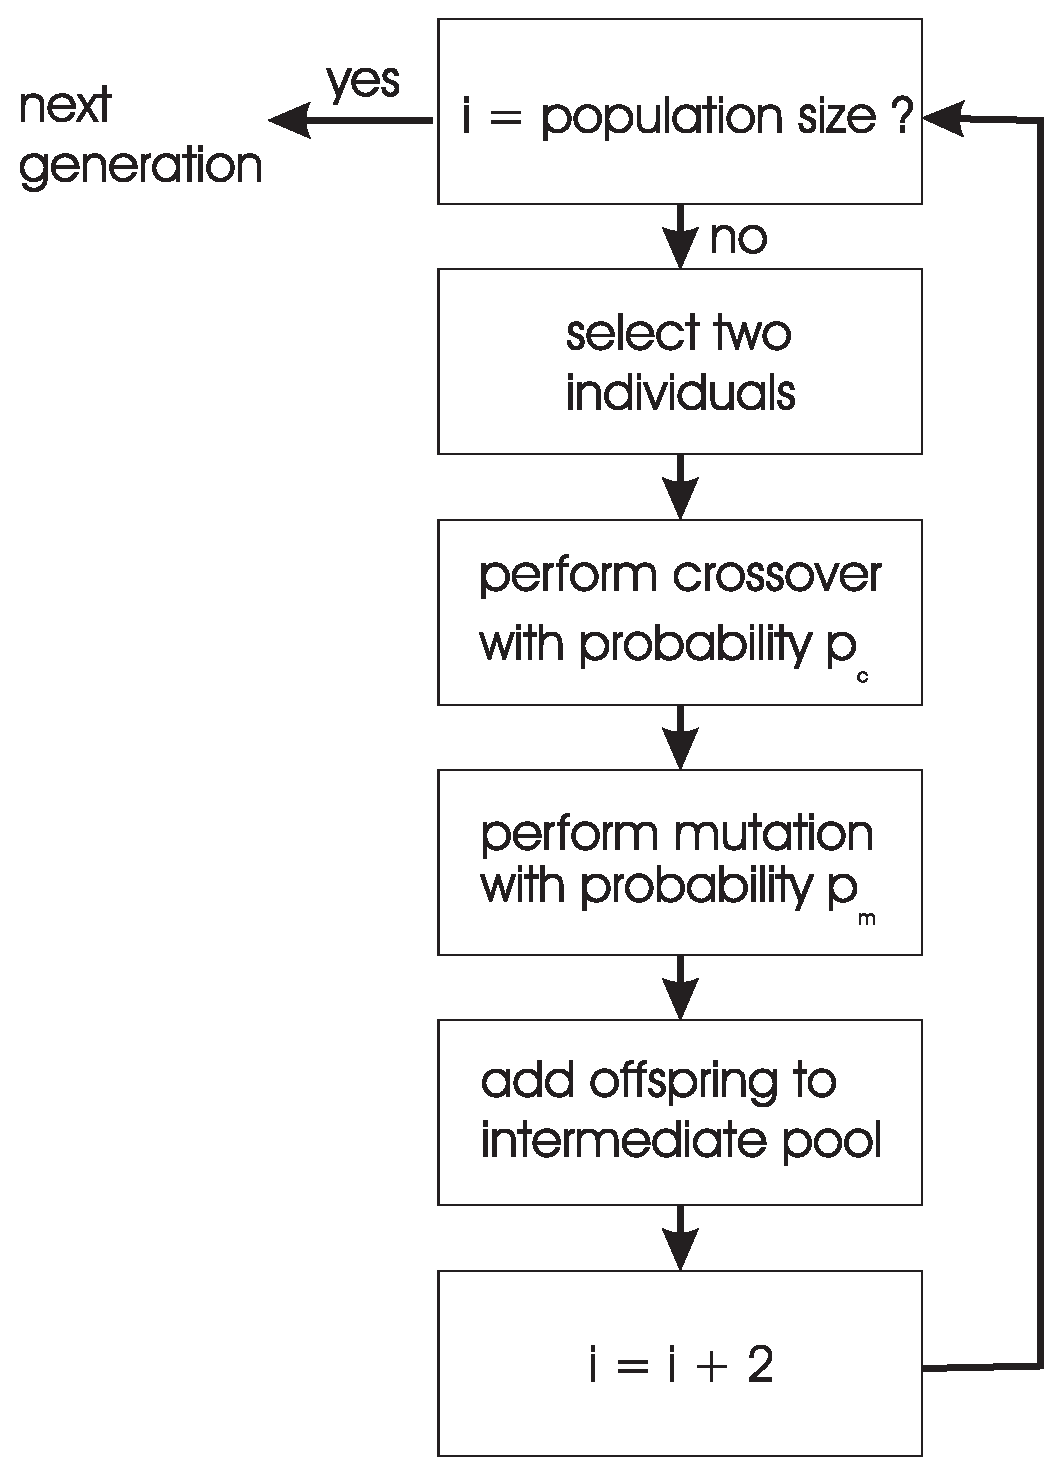
\includegraphics[height=0.5\linewidth]{figs/gaflowchart.eps}
	\end{center}
\end{frame}

\subsection{Representation}
\begin{frame}{Genetic Algorithms}{Representation: Binary}
	\vspace{-0.3cm}
	\begin{table}[]
	\centering
	\begin{tabular}{|l|l|l|l|l|l|l|l|l|}
	\hline
 	1 & 1 & 0 & 1 & 0 & 0 & 0 & 1\\ \hline
	\end{tabular}
	\end{table}

	One of the oldest and widely used codifications
	\begin{itemize}
		\item Consequence of Holland's Theorem
		\item Strong historical influence
  	\end{itemize}
	Often used to codify non-binary information (not recommended)
	\begin{itemize}
		\item Pure binary codification
		\item Gray coding
		\item Custom codification
	\end{itemize}
	\vspace{-1.5cm}
	\hfill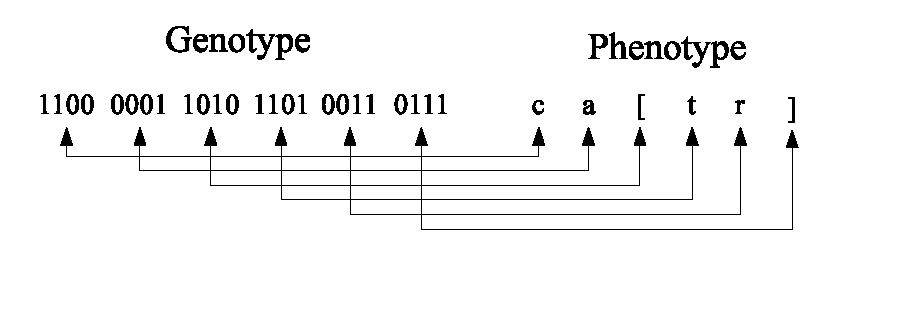
\includegraphics[width=0.55\linewidth]{figs/coding.eps}\\
	\vspace{-0.3cm}
	Hint: Use binary codification to represent binary information
\end{frame}

\begin{frame}{Genetic Algorithms}{Representation: Integer}
	\begin{table}[]
	\centering
	\begin{tabular}{|l|l|l|l|l|l|l|l|l|}
	\hline
 	4 & 3 & 2 & 1 & 0 & 4 & 2 & 3 & 3\\ \hline
	\end{tabular}
	\end{table}

	Chomosome as a sequence of integers
	\begin{itemize}
		\item More natural codification for many problems
		\item Optimization of integer values
		\item Integer representation ($\{1,2,3,4\}=\{North,East,South,West\}$)
  	\end{itemize}
\end{frame}

\begin{frame}{Genetic Algorithms}{Representation: Floating-point}
	\begin{table}[]
	\centering
	\begin{tabular}{|l|l|l|l|l|l|l|l|l|}
	\hline
 	1.1 & 0.2 & 3.0 & 33.2 & 0.0 & -3.2 & 130.1 & 88.3 & -7.1\\ \hline
	\end{tabular}
	\end{table}

	Chomosome as a sequence of floating-point values
	\begin{itemize}
		\item Common in optimization problems
		\item Solutions with continous nature
  	\end{itemize}
\end{frame}

\IfStrEq{\modo}{MASTER-INDUSTRIALES}{
\begin{frame}{Genetic Algorithms}{Representation: Floating point (II)}
	\vspace{-0.2cm}

	\begin{center}
	ANN encoding with a GA\\\bigskip
	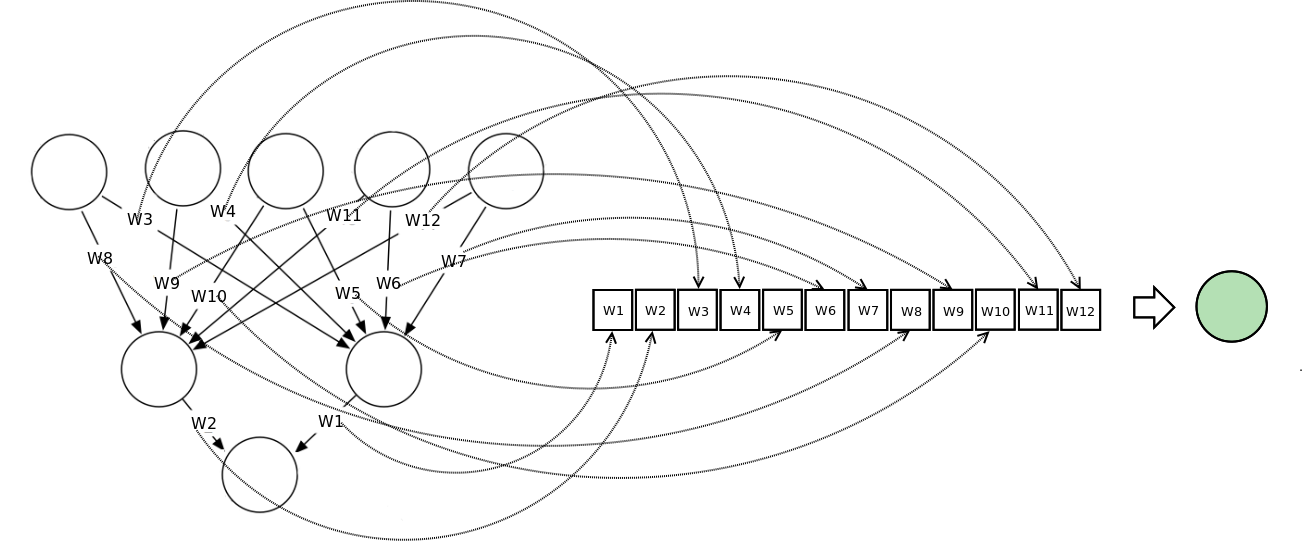
\includegraphics[width=0.85\linewidth]{figs/ann-ga.png}\\
	\tiny{\href{http://www.turingfinance.com/misconceptions-about-neural-networks/}{(Source)}}
	\end{center}
\end{frame}
}{}

\begin{frame}{Genetic Algorithms}{Representation: Permutation}
	\vspace{-0.7cm}
	\begin{table}[]
	\centering
	\begin{tabular}{|l|l|l|l|l|l|}
	\hline
 	4 & 3 & 2 & 5 & 6 & 1 \\ \hline
	\end{tabular}
	\end{table}

	\vspace{-0.2cm}

    \begin{columns}
 	   \column{.50\textwidth}
	Some problems involve order
	\begin{itemize}
		\item Sequence of integers
		\item No repeated numbers
		\item Range of valid numbers
		\item Special genetic operators
  	\end{itemize}
	Information can be contained in
	\begin{itemize}
		\item The locus (position)
		\begin{itemize}
		\item[] $[3,1,2,4] \Rightarrow [C,A,B,D]$
		\end{itemize}
		\item The allele (value)
		\begin{itemize}
		\item[] $[3,1,2,4] \Rightarrow [B,C,A,D]$
		\end{itemize}
	\end{itemize}
 	   \column{.50\textwidth}
	\begin{center}
	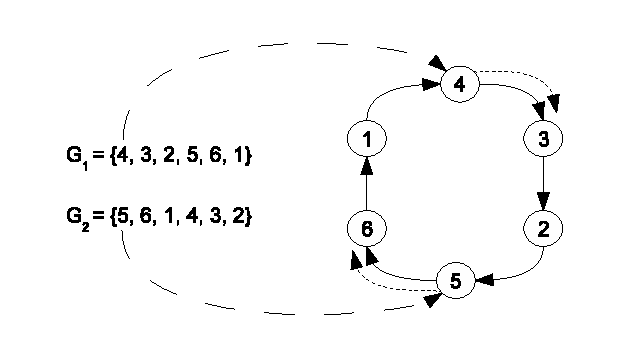
\includegraphics[width=\linewidth]{figs/codification.eps}\\
	\small{Integer codification to solve TSP}
	\end{center}
	\end{columns}
	\note{Ejemplo con planificacion de tareas}
\end{frame}

\subsection{Mutation}
\begin{frame}{Genetic Algorithms}{Mutation}
	\textbf{Mutation}: Genetic operator that uses one parent
	\begin{itemize}
		\item Introduces randomness into the genotype
		\item Depends on representation
  	\end{itemize}
	Main objectives
	\begin{itemize}
		\item Avoid local minima (premature convergence)
		\item Enhances exploration
	\end{itemize}
	Often dependent on the \alert{mutation rate}
	\begin{itemize}
		\item Significant influence in the algorithm behaviour
		\item Higher mutation rate, higher exploration
	\end{itemize}
\end{frame}

\begin{frame}{Genetic Algorithms}{Mutation for binary representations}
	Flip bit with probability $p_m$
	\vspace{-0.7cm}
	\begin{center}
	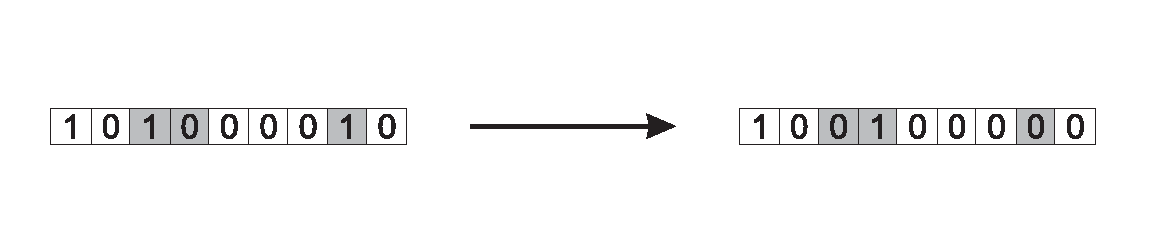
\includegraphics[width=0.8\linewidth]{figs/flip.eps}
	\end{center}
	\vspace{-0.7cm}
	Optimal $p_m$ depends on the problem and goals
	\begin{itemize}
		\item Need of high fitness population
		\item Need of high fitness individual
		\item Need of genetic diversity
		\item Modality of the problem
		\item Algorithm dynamics
  	\end{itemize}
	Rule of thumb: $p_m = \frac{1}{length}$
\end{frame}

\begin{frame}{Genetic Algorithms}{Mutation for integer representations}
	Two main mutations applied to each gene
	\begin{itemize}
		\item \textbf{Random resetting}: Choose new random value with $p_m$
		\item \textbf{Creep mutation}: Add small (positive or genative) random value with $p_m$
	\end{itemize}
\end{frame}

\begin{frame}{Genetic Algorithms}{Mutation for floating-point representations}
	Set new value with value drawn from a distribution
	\begin{itemize}
		\item \textbf{Uniform mutation} Choose new random value from $[L, U]$ with $p_m$
		\item \textbf{Non-uniform mutation} Usually adding a value drawn from a zero-mean gaussian  distribution
	\end{itemize}
	\begin{center}
	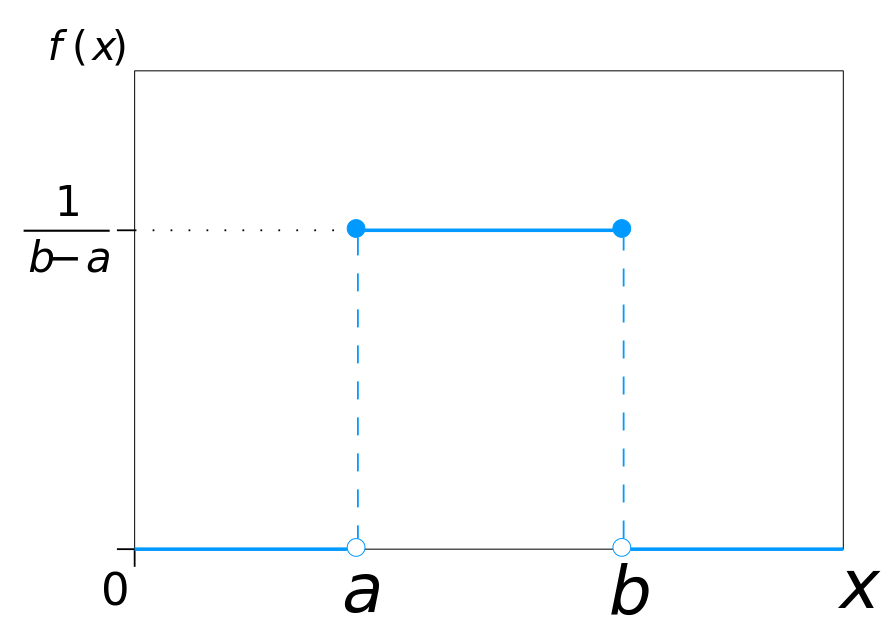
\includegraphics[width=0.4\linewidth]{figs/uniform.png}
	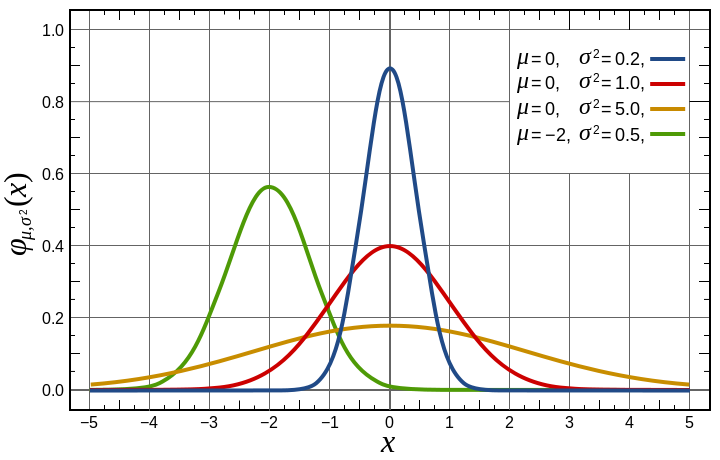
\includegraphics[width=0.4\linewidth]{figs/gaussian.png}
	\end{center}
\end{frame}

\begin{frame}{Genetic Algorithms}{Mutation for permutation representations}
	Genes are no longer independent
	\begin{itemize}
		\item No gene mutation, $p_m$ affects the whole chromosome
	\end{itemize}
    \begin{columns}
 	   \column{.50\textwidth}
		\begin{center}
		Swap mutation\\
		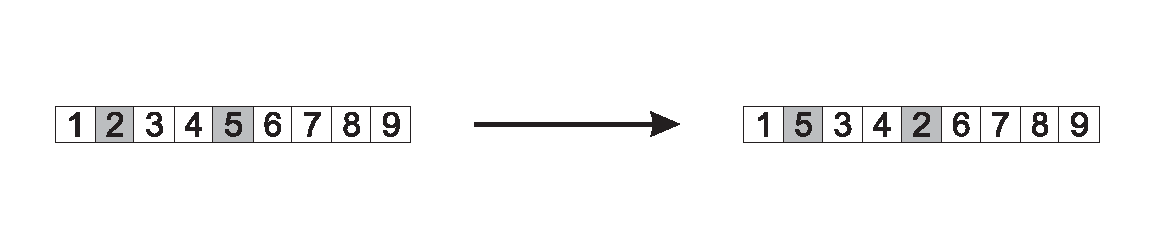
\includegraphics[width=\linewidth]{figs/swap.eps}\\
		Scramble mutation\\
		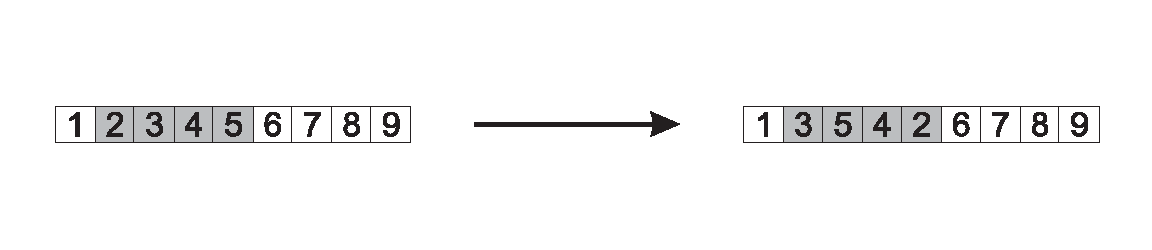
\includegraphics[width=\linewidth]{figs/scramble.eps}\\
		\end{center}
 	\column{.50\textwidth}
		\begin{center}
		Insert mutation\\
		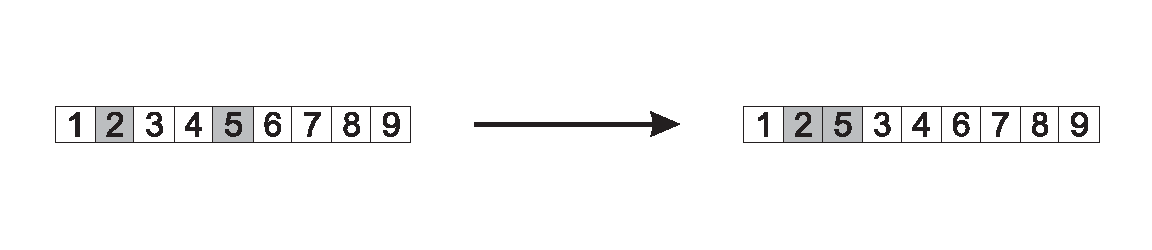
\includegraphics[width=\linewidth]{figs/insert.eps}\\
		Inversion mutation\\
		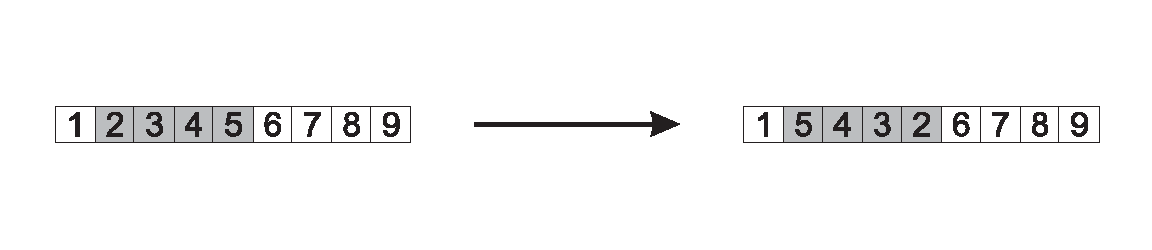
\includegraphics[width=\linewidth]{figs/inversion.eps}\\
		\end{center}
	   \end{columns}
\end{frame}

\subsection{Recombination}
\begin{frame}{Genetic Algorithms}{Recombination}
	Recombination creates one individual from two or more parents
	\begin{itemize}
		\item Also known as crossover (specially for two parents)
		\item Basic feature in GA
		\item Parents selection mechanism needed
	\end{itemize}
	Usually applied to all new individuals
	\begin{itemize}
		\item Not used when elitism is applied
		\item Sometimes applied with $p_c \in [0.5, 1]$ 
	\end{itemize}
	Objectives of recombination
	\begin{itemize}
		\item Combine parents' behavior $\Rightarrow$ No new genetic material
		\item Constructive role
		\item Enhances explotation
	\end{itemize}
\end{frame}

\begin{frame}{Genetic Algorithms}{Recombination: Binary and integer representations}
	Three crossover mechanisms for binary and integer encodings
    \begin{columns}
 	   \column{.50\textwidth}
		\begin{center}
		One-point crossover\\
		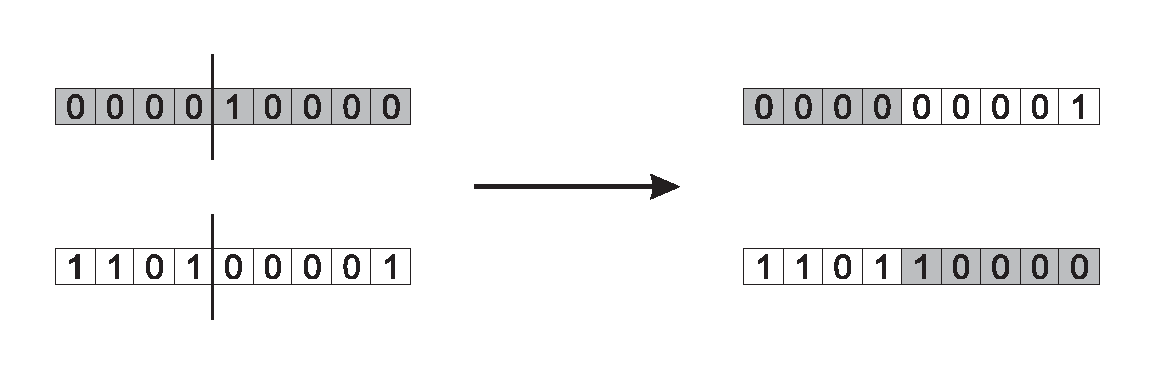
\includegraphics[width=\linewidth]{figs/onepoint.eps}\\
		\end{center}
 	\column{.50\textwidth}
		\begin{center}
		Two-points crossover\\
		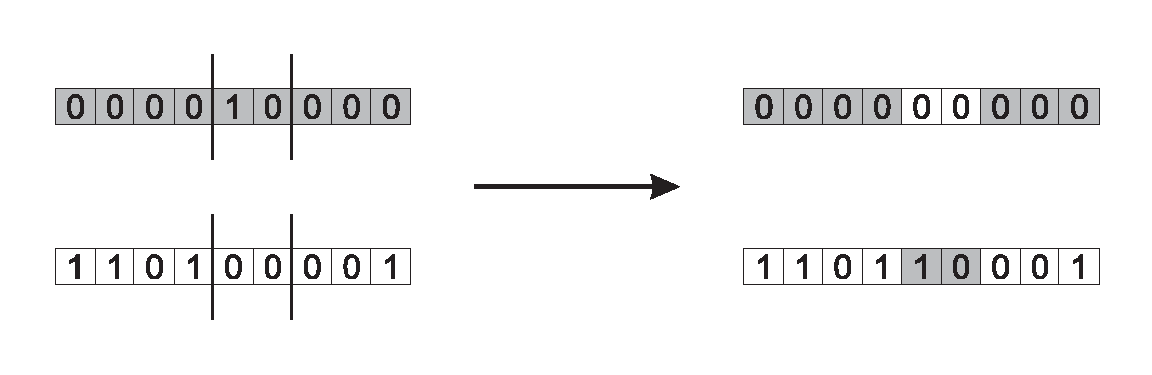
\includegraphics[width=\linewidth]{figs/npoint.eps}\\
		\end{center}
	   \end{columns}

	\begin{center}
		\centering Uniform crossover\\
		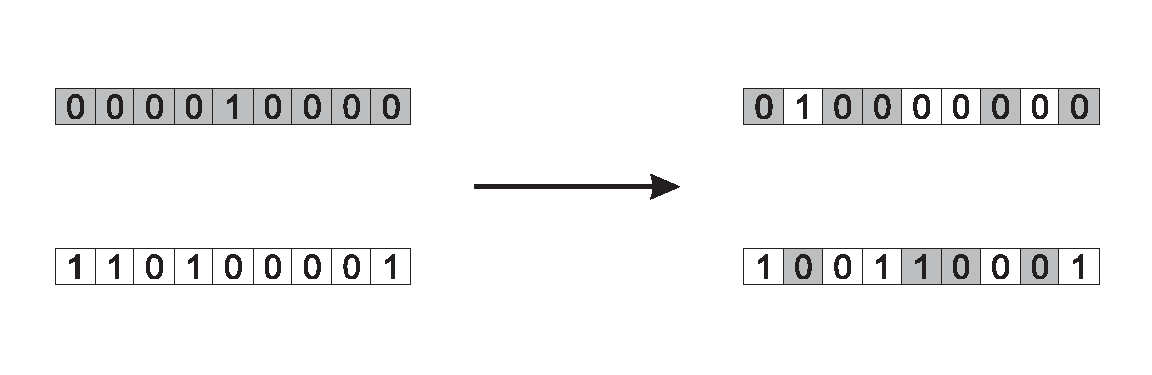
\includegraphics[width=0.5\linewidth]{figs/uniform-xover.eps}
	\end{center}

	\note{Hablar de positional bias y distributional bias}
\end{frame}

\begin{frame}{Genetic Algorithms}{Recombination: Floating point representations (I)}
	Discrete recombination
	\begin{itemize}
		\item Analogous to binary recombination
		\item No new genetic material
	\end{itemize}
	Arithmetic recombination
	\begin{itemize}
		\item Combines the parents' genes
		\item Weighted sums of genes: $z_i=\alpha x_i + (1-\alpha) y_i$
		\item Usually, $\alpha=0.5$ (average values)
		\item Different arithmetic recombinations
	\end{itemize}
\end{frame}

\begin{frame}{Genetic Algorithms}{Recombination: Floating point representations (II)}
	\vspace{-0.75cm}
	\begin{center}
	Whole arithmetic recombination\\
	\footnotesize{(All genes are included)}\\
	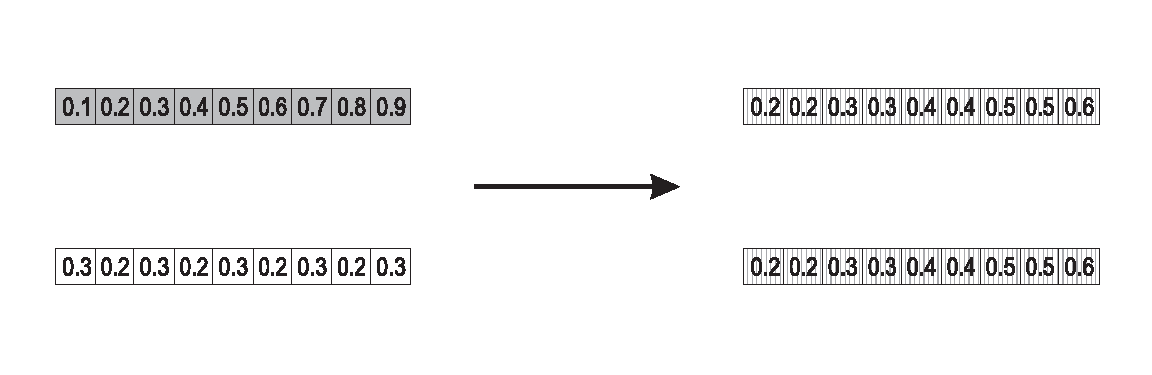
\includegraphics[width=0.5\linewidth]{figs/wholearithmetic.eps}\\
	\end{center}
	\vspace{-0.5cm}

    \begin{columns}
 	   \column{.50\textwidth}
		\begin{center}
		Simple arithmetic recombination\\
		\footnotesize{(Similar to one-point crossover)}
		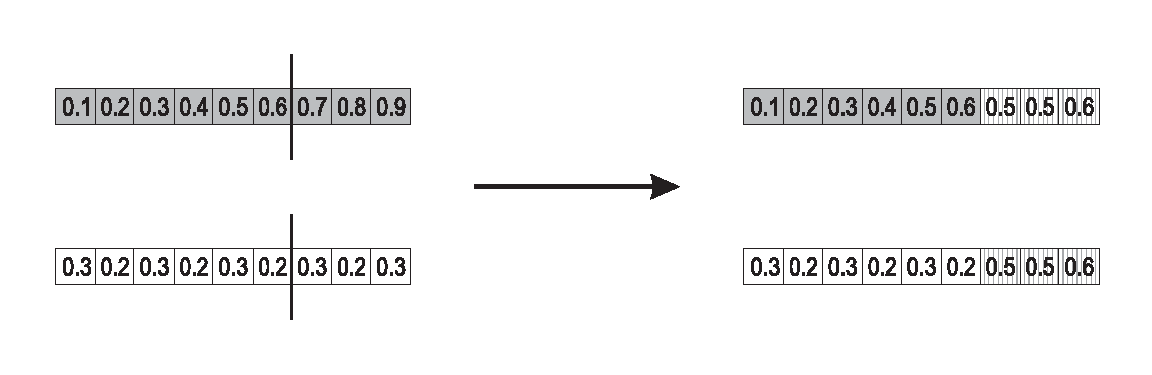
\includegraphics[width=\linewidth]{figs/simplearithmetic.eps}\\
		\end{center}
 	   \column{.50\textwidth}
		\begin{center}
		Single arithmetic recombination\\
		\footnotesize{(Similar to uniform crossover)}
		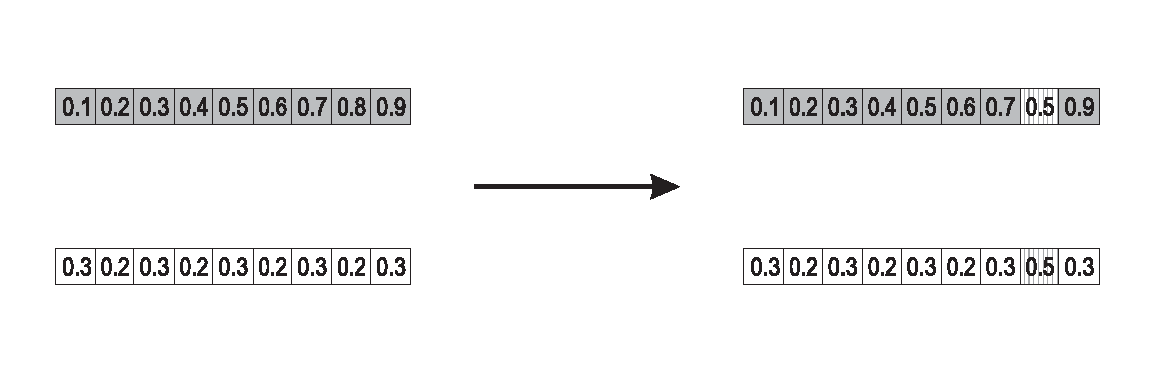
\includegraphics[width=\linewidth]{figs/singlearithmetic.eps}\\
		\end{center}
		\end{columns}
\end{frame}

\begin{frame}{Genetic Algorithms}{Recombination: Permutation representations}
    \begin{columns}
 	   \column{.50\textwidth}
		Specialized recombinations
		\begin{itemize}
		\item Partially Mapped Crossover
		\item Edge Crossover
		\item Order Crossover
		\item Cycle Crossover
		\end{itemize}

	    \column{.50\textwidth}
		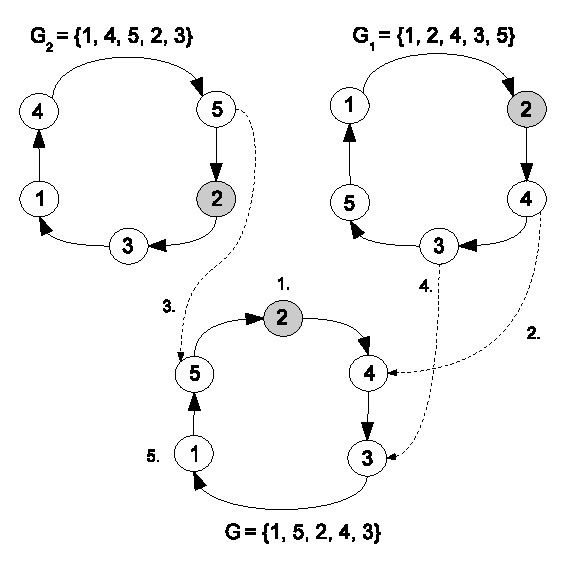
\includegraphics[width=\linewidth]{figs/permutation-xover.eps}
	\end{columns}
\end{frame}

\subsection{Selection}
\begin{frame}{Genetic Algorithms}{Selection}
	Two purposes for selection
	\begin{itemize}
		\item Parent selection: Individuals to generate offspring
		\item Survivor selection: Individuals to remplace
  	\end{itemize}
	Usually same methods applied to both
\end{frame}

\begin{frame}{Genetic Algorithms}{Selection: Fitness Proportional Selection}
    \begin{columns}
 	   \column{.60\textwidth}
	Selection probability proportional to fitness 
	\begin{itemize}
		\item Premature convergence
		\item Lack of selective pressure for close fitness values
		\item Selective pressure not customizable
		\item Susceptibility to function transposition
  	\end{itemize}
	Historically relevant
	    \column{.40\textwidth}
	\begin{center}
    \begin{columns}
 	   \column{.60\textwidth}
	\begin{block}{}
	$p_s = \frac{f_i}{\sum_{j=1}^\mu f_j}$
	\end{block}
	\end{columns}
	\bigskip
	\includegraphics[width=\linewidth]{figs/fps.eps}
	\end{center}
	\end{columns}
\end{frame}

\begin{frame}{Genetic Algorithms}{Selection: Ranking Selection}
    \begin{columns}
 	   \column{.60\textwidth}
	Selection probability proportional to rank
	\begin{itemize}
		\item Individuals are sorted by fitness
		\item Arbitrary rank to probability mapping
		\item Avoid problems with super individuals
		\item Selective pressure independent of fitness
		\item Selective pressure not customizable
  	\end{itemize}
	    \column{0.4\textwidth}
	\begin{center}
	\small{
	\begin{block}{Linear mapping}
	\begin{equation*}
	P_{lin_rank}(i)=\frac{(2-s)}{\mu} + \frac{2i(s-1)}{\mu (\mu -1)}
	\end{equation*}
	$1.0 < s < 2.0$
	\end{block}

	\begin{block}{Exponential mapping}
	$P_{exp_rank}(i)=\frac{1-e^{-i}}{c}$\\
	c = normalization factor
	\end{block}
	}
	\end{center}
	\end{columns}
\end{frame}

\begin{frame}{Genetic Algorithms}{Selection: Tournament Selection}
    \begin{columns}
 	   \column{.50\textwidth}
	   \begin{block}{Algorithm of tournament size $k$}
	\begin{enumerate}
		\item Select randomly $k$ chromosomes
		\item Compute their fitness
		\item Select the fittest one
		\item Go to 1
  	\end{enumerate}
	\end{block}
 	   \column{.50\textwidth}
	Customizable selective pressure
	\begin{itemize}
		\item Depends on $k$ and $\mu$
	\end{itemize}
	De facto standard
	\begin{itemize}
		\item Good for parallel computation
		\item Efficient implementation
	\end{itemize}
	Usually $k=2$ in GA, in GP $k=7$
	\end{columns}
\end{frame}

\begin{frame}{Genetic Algorithms}{Selection: Survival selection}
	Two strategies
	\begin{itemize}
		\item Generational (all the population is remplaced)
		\item Steady-stade (partial remplacement)
	\end{itemize}
	Survival selection algorithms
	\begin{itemize}
		\item Fitness-Based Replacement (inverse of the previous ones)
		\item Age-Based Replacement
		\item Elitism
  	\end{itemize}
\end{frame}

\section{Genetic Programming}
\subsection{Introduction}
\begin{frame}{Genetic Programming}{Introduction (I)}
    \begin{columns}
 	   \column{.70\textwidth}
	GP is a family of algorithms
	\begin{itemize}
		\item Evolve programs
		\item Self-programming computers
		\item GP, Linear GP, Cartesian GP, EDA, ...
	\end{itemize}

	GP introduced by Koza in the 90's
	\begin{itemize}
		\item[] \small{Koza, J.R.  ``\textit{Genetic Programming: On the Programming of Computers by Means of Natural Selection}'', MIT Press. 1992}
	\end{itemize}

	GA and ES focused on optimization
	\begin{itemize}
		\item GP focused on Machine Learning
	\end{itemize}
 	   \column{.30\textwidth}
	   \begin{center}
	   Optimization\\
	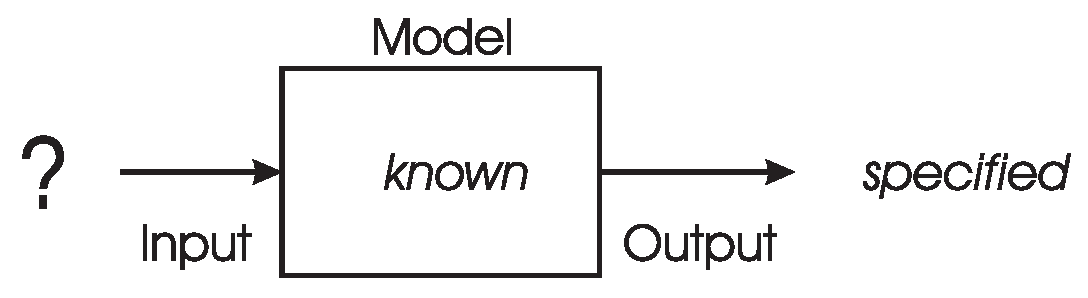
\includegraphics[width=\linewidth]{figs/optimization.eps}\\\bigskip
		Modelling\\
	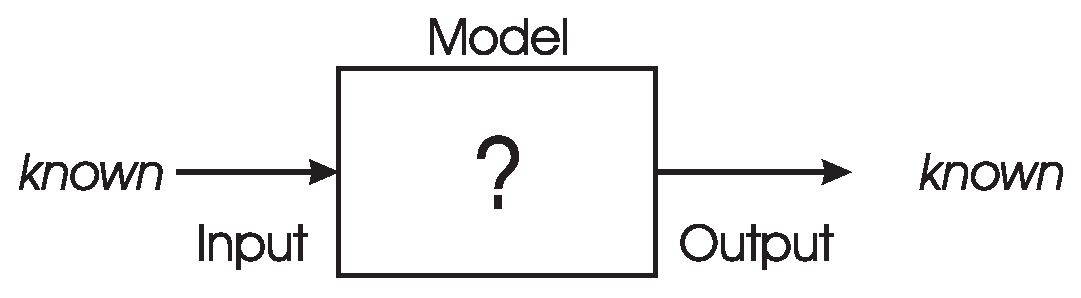
\includegraphics[width=\linewidth]{figs/modelling.eps}\\\bigskip
		Simulation\\
	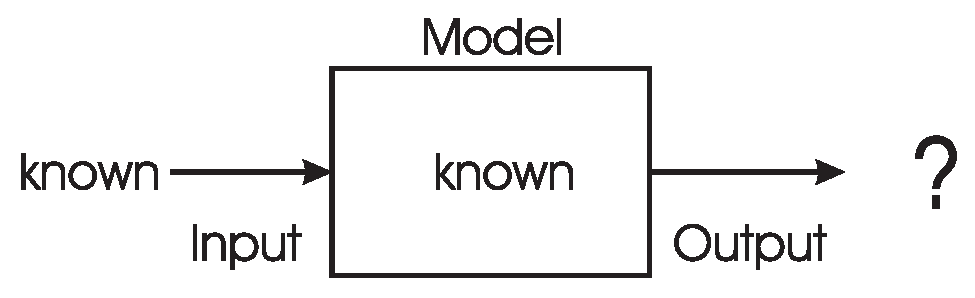
\includegraphics[width=\linewidth]{figs/simulation.eps}\\
	\end{center}
	   \end{columns}
\end{frame}

\begin{frame}{Genetic Programming}{Introduction (II)}
	Example: Credit scoring problem within a bank.  Develop a model describing good customers

	\begin{table}[]
	\centering
		\begin{tabular}{|l|l|l|l|l|}
		\hline
		Id 	 & Children & Salary & Status & Credit \\ \hline
 		Id-1 & 2 	& 45.000 & Married & 0 \\ \hline
  		Id-2 & 0 	& 30.000 & Single & 1 \\ \hline
   		Id-3 & 1 	& 40.000 & Married & 1 \\ \hline
   		Id-4 & 2 	& 60.000 & Divorced & 1 \\ \hline
   		 ... &  	&  &  &  \\ \hline
   		Id-X & 2 	& 50.000 & Married & 1  \\ \hline
		\end{tabular}
	\end{table}

	   Possible model:\\
	   \texttt{IF (children=2) AND (Salary>80.000) THEN good ELSE bad}
\end{frame}

\begin{frame}{Genetic Programming}{Introduction (III)}
    \begin{columns}
 	   \column{.50\textwidth}
	  	General form\\
			\begin{center}
	   		\texttt{IF (Formula) \\THEN good \\ELSE bad}\\
	  		\end{center} 
	   In EC terms\\
	   Phenotype: Formula\\
	   Fitness: Classification accuracy
 	   \column{.50\textwidth}
		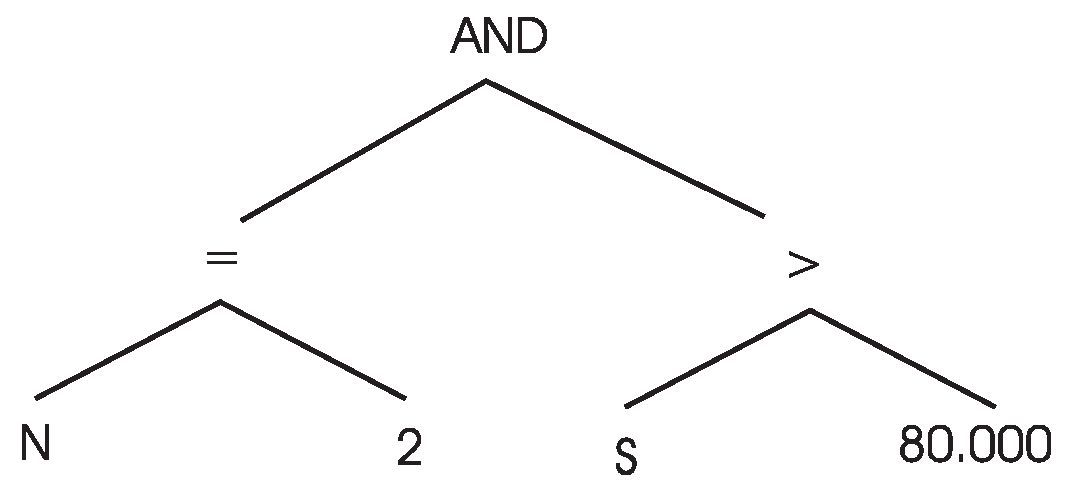
\includegraphics[width=\linewidth]{figs/parsetree.eps}\\\bigskip
	   \centering\small{\texttt{(children=2) AND (Salary>80.000)}}
	\end{columns}
\end{frame}

\subsection{Representation}
\begin{frame}{Genetic Programming}{Representation (I)}
	GP representation differs in two aspects
	\begin{itemize}
		\item Nonlinear structure
		\item Variable size
	\end{itemize}
	New representation and genetic operators
	\begin{itemize}
		\item Same selection (done in phenotipic space)
	\end{itemize}
\end{frame}

\begin{frame}[fragile]{Genetic Programming}{Representation (II)}
    \begin{columns}
 	   \column{.330\textwidth}
	   		\begin{center}
	    	Arithmetic formula
			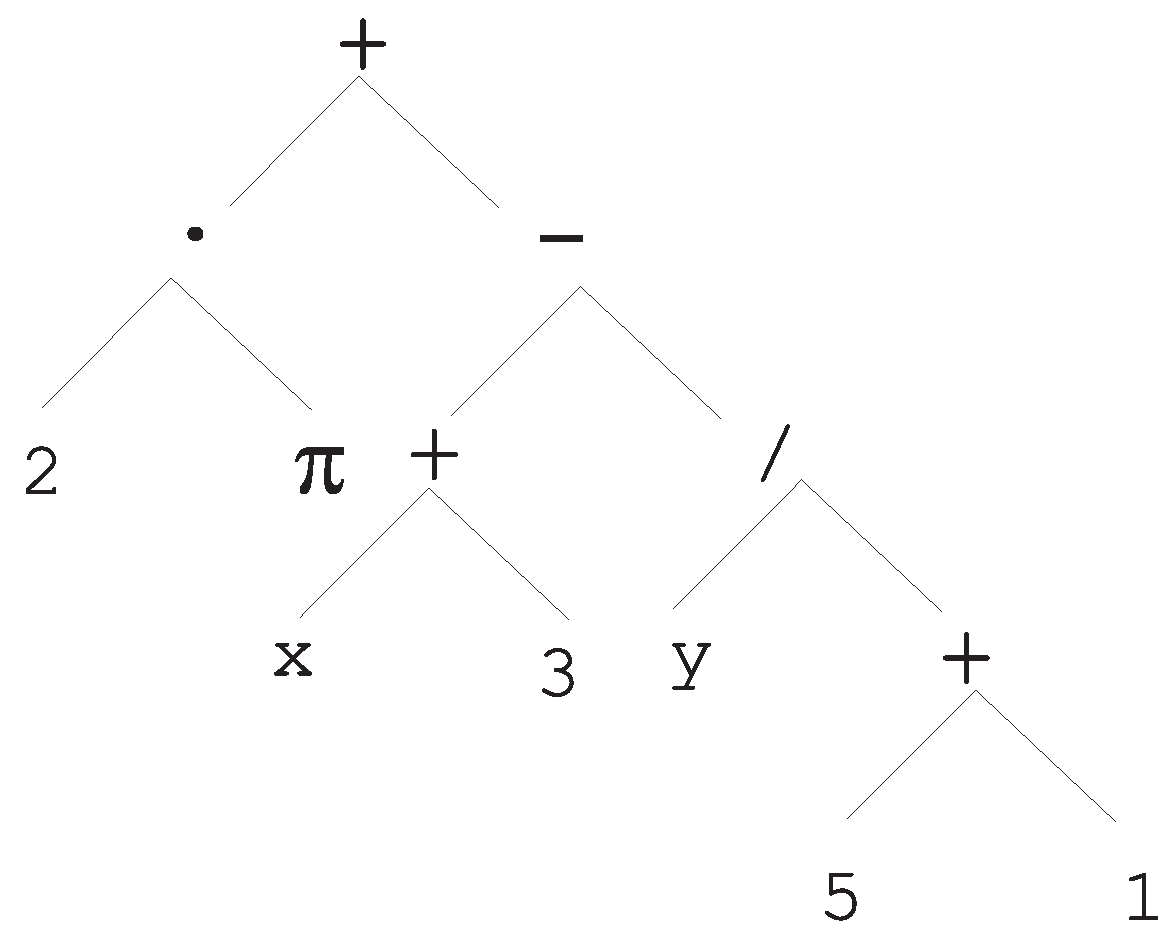
\includegraphics[width=\linewidth]{figs/arithmetictree.eps}\\
			\begin{equation*}
			\bigg( 2\pi + \big((x+3)-\frac{y}{5+1}\big)\bigg)
			\end{equation*}	
			\end{center}
 	   \column{.330\textwidth}
	   		\begin{center}
	    	Logical formula
			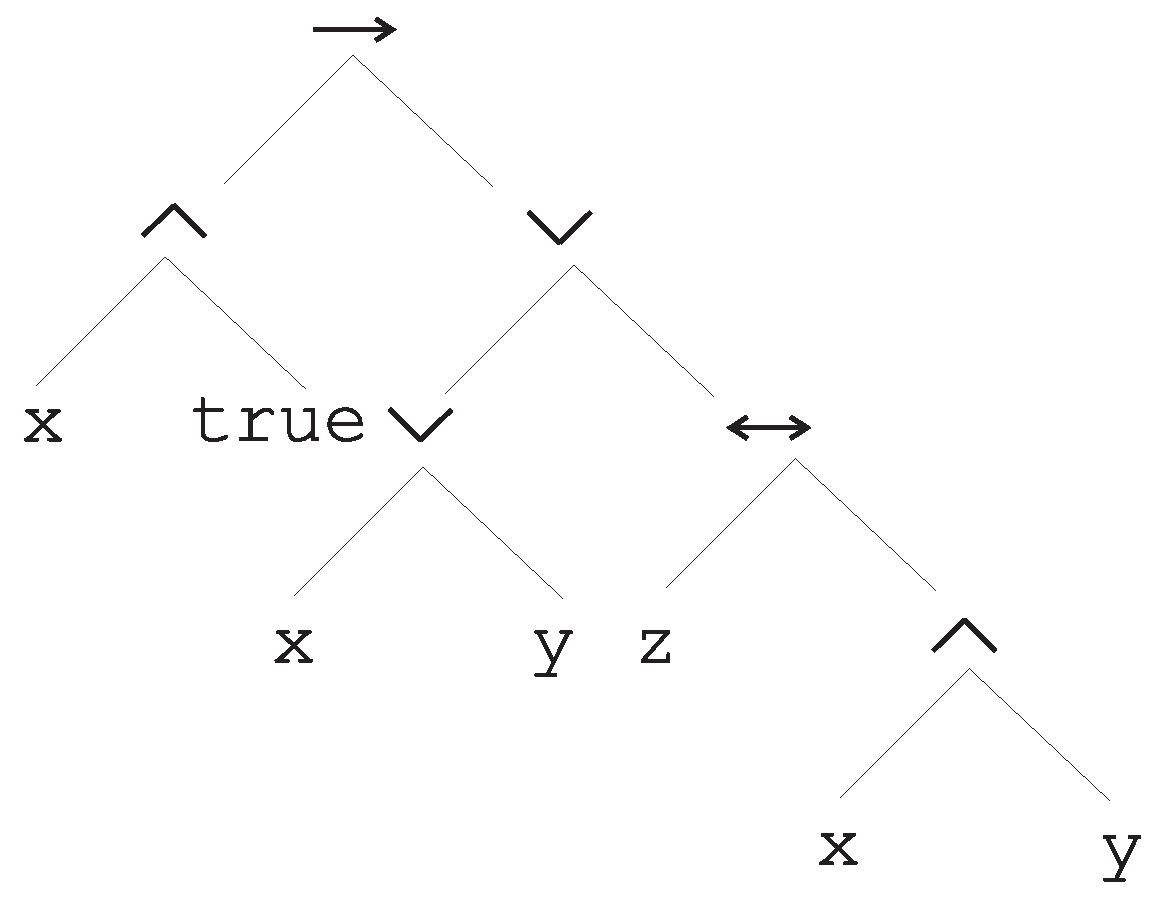
\includegraphics[width=\linewidth]{figs/logicaltree.eps}\\
			\begin{multline*}
			(x	\wedge true) \to \\((x \vee y) \vee (z \leftrightarrow (x\vee y)))
			\end{multline*}	
			\end{center}
 	   \column{.330\textwidth}
	   		\begin{center}
	    	Program
			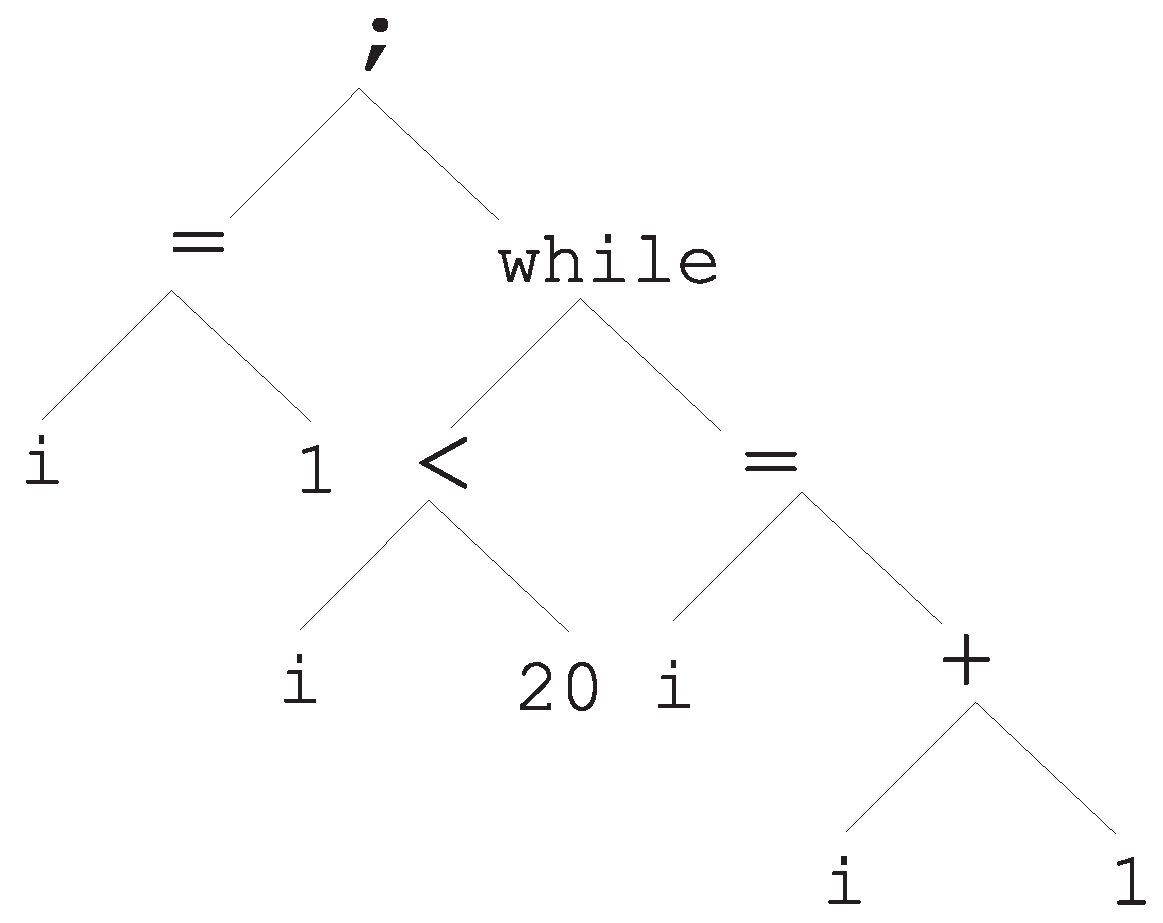
\includegraphics[width=\linewidth]{figs/programtree.eps}\\
			\begin{verbatim}
			i=1;
			while (i<20) {
				i = i+1;
			}
			\end{verbatim}	
			\end{center}
	\end{columns}
\end{frame}

\begin{frame}[fragile]{Genetic Programming}{Representation (III)}
	Two types of nodes
	\begin{itemize}
		\item \textbf{Function set} Internal nodes. It has an ssociated number of attributes
		\item \textbf{Terminal set} Leaves of the tree
	\end{itemize}
	Danger: Inviable trees
	\begin{itemize}
		\item Grammar-aware GP variants
		\item Strongly Typed Genetic Programming (STGP), Grammatical Evolution (GE), ...
	\end{itemize}
	\href{http://www.genetic-programming.com/gpcircuitanimation.gif}{(Complex representation example)}
\end{frame}

\subsection{Mutation}
\begin{frame}{Genetic Programming}{Mutation (I)} 
	Application of genetic operators in GP contrast to GA
	\begin{center}
		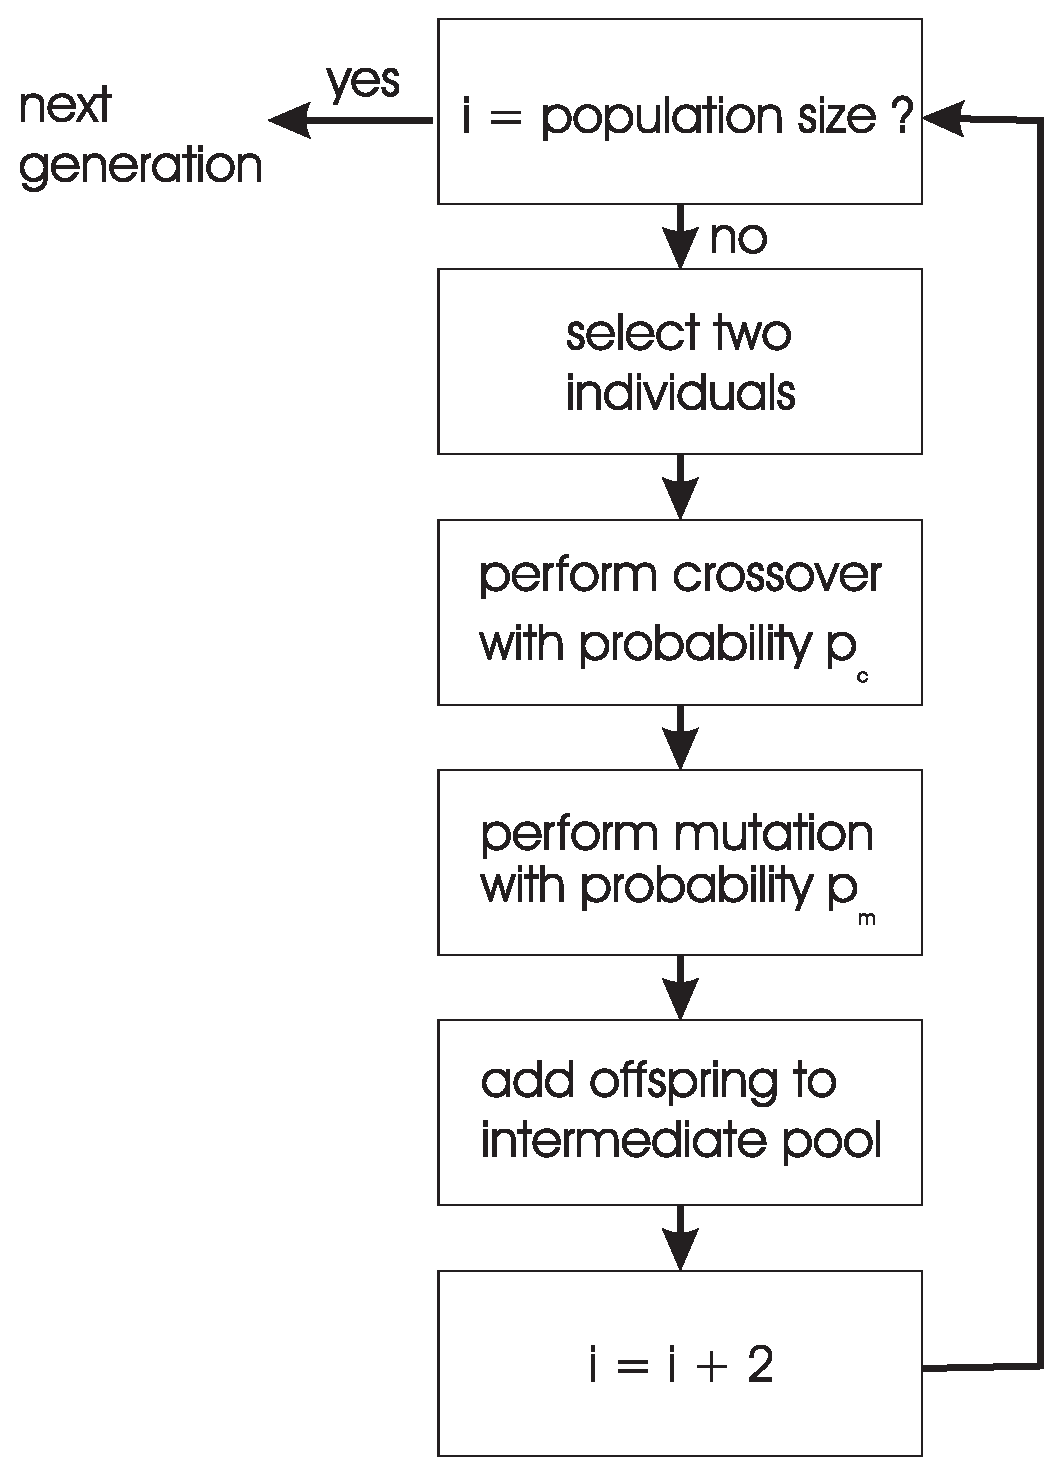
\includegraphics[height=0.45\linewidth]{figs/gaflowchart.eps} \quad\quad
		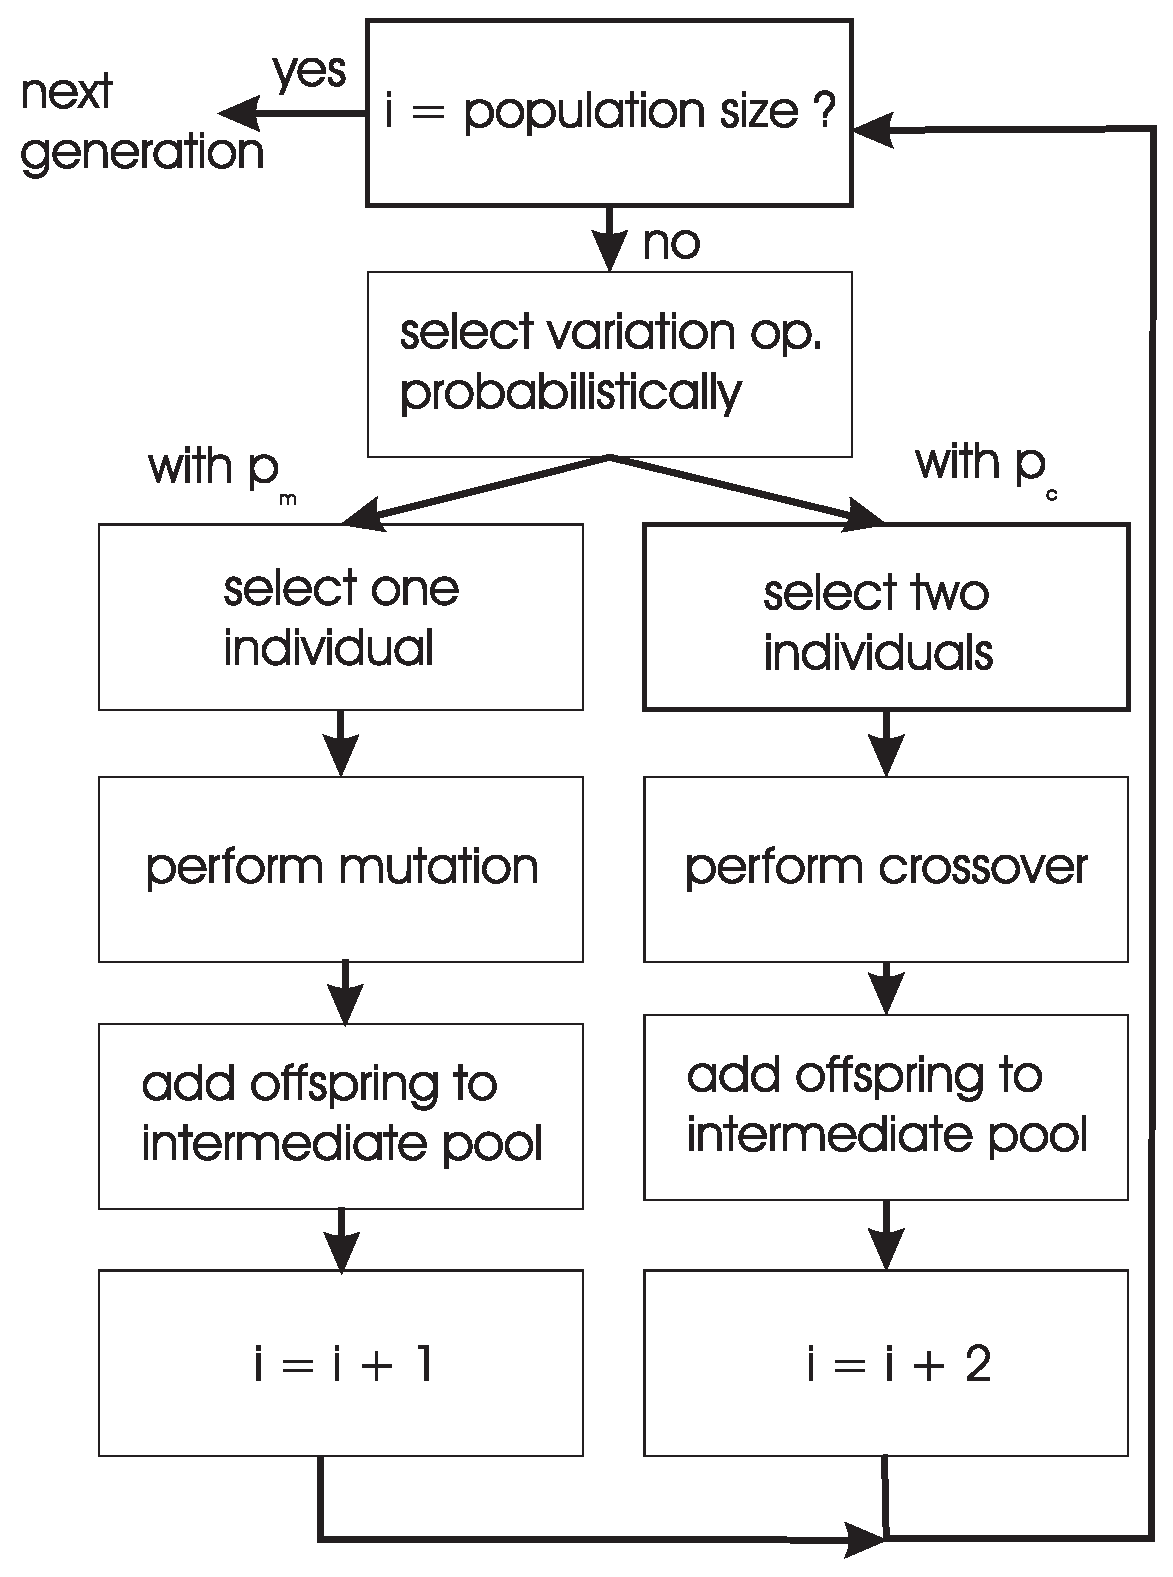
\includegraphics[height=0.45\linewidth]{figs/gpflowchart.eps}
	\end{center}
\end{frame}

\begin{frame}{Genetic Programming}{Mutation (II)} 
    \begin{columns}
 	   \column{.50\textwidth}
	\textbf{Subtree mutation}
	\begin{enumerate}
		\item Select a random node
		\item Delete subtree
		\item Add new random subtree
	\end{enumerate}

 	   \column{.50\textwidth}
	Parameters
	\begin{itemize}
		\item Probability of choosing a terminal node
	\end{itemize}

	Highly correlated with \alert{code bloat}
	\end{columns}

	\bigskip

    \begin{columns}
 	   \column{.15\textwidth}
 	   \column{.30\textwidth}
		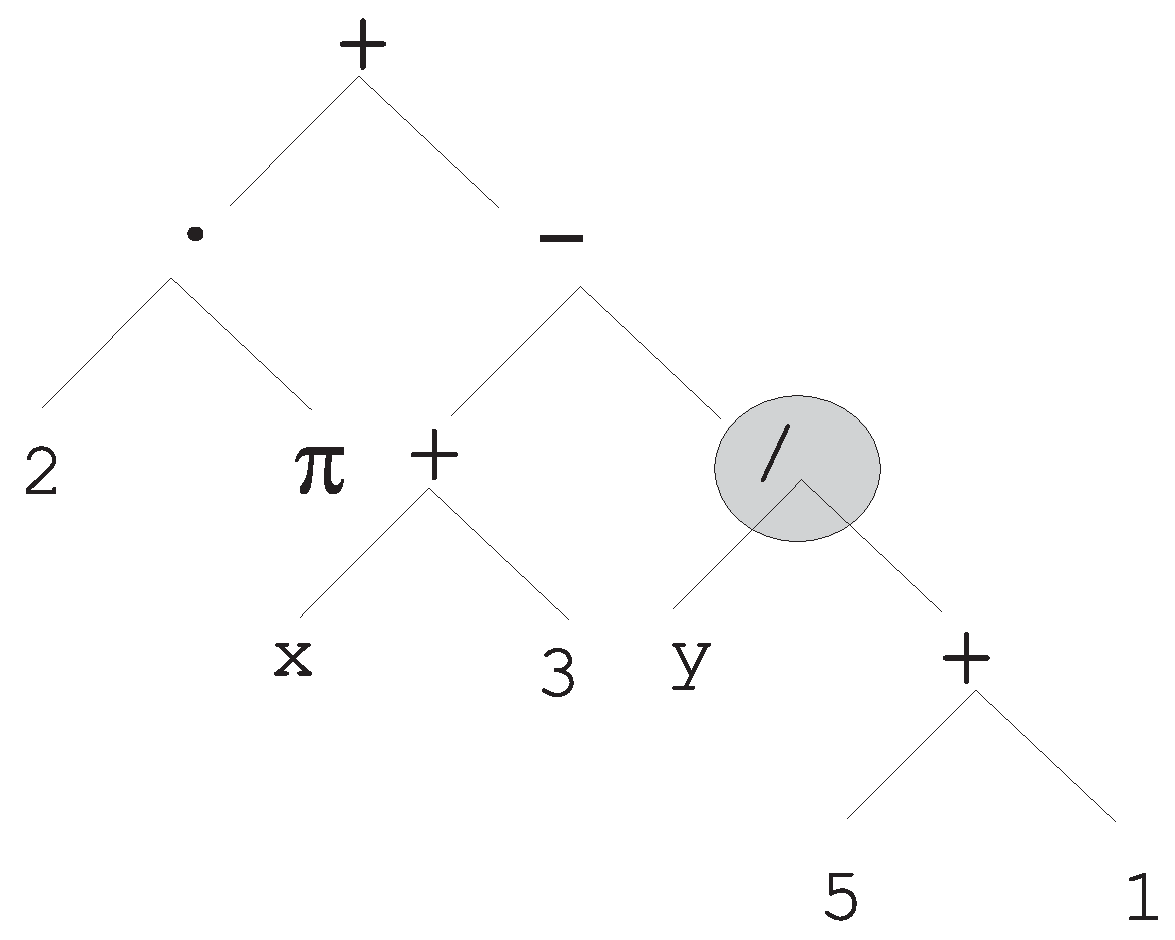
\includegraphics[width=\linewidth]{figs/gpparentmutation.eps} 
 	   \column{.05\textwidth}
		$\Rightarrow$ 
 	   \column{.30\textwidth}
		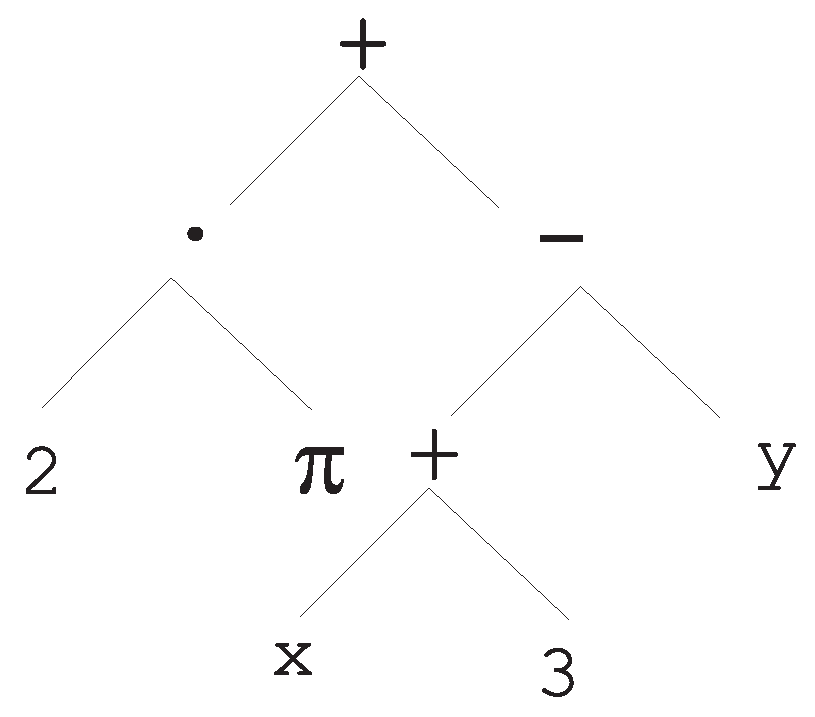
\includegraphics[width=\linewidth]{figs/gpchildmutation.eps}
 	   \column{.15\textwidth}
	\end{columns}
\end{frame}

\begin{frame}{Genetic Programming}{Mutation (III)} 
	Alternative mutation operators
	\begin{itemize}
		\item Size-fair subtree mutation
		\item Node replacement mutation (point mutation)
		\item Hoist mutation
		\item Shrink mutation
	\end{itemize}
\end{frame}

\subsection{Recombination}

\begin{frame}[fragile]{Genetic Programming}{Recombination (I)}
    \begin{columns}
 	   \column{.50\textwidth}
			Subtree crossover
			\begin{enumerate}
				\item Take a random node from both parents
				\item Swap subtrees
			\end{enumerate}
			Parameters
			\begin{itemize}
				\item Probability of choosing a terminal node
			\end{itemize}

 	   \column{.50\textwidth}
    		\begin{columns}
 	   			\column{.5\textwidth}
					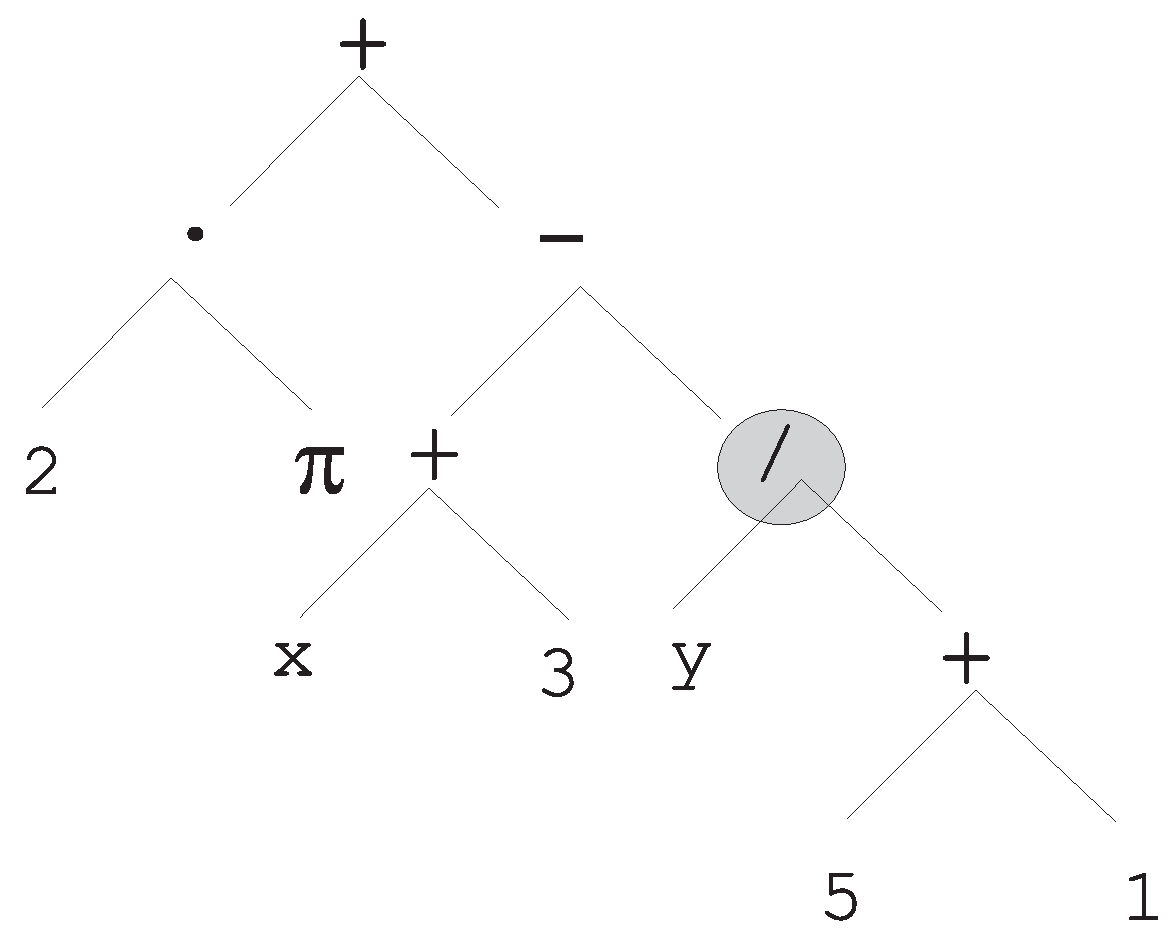
\includegraphics[width=\linewidth]{figs/gpparentacrossover.eps} 
 	   			\column{.02\textwidth}
					+
 	   			\column{.5\textwidth}
					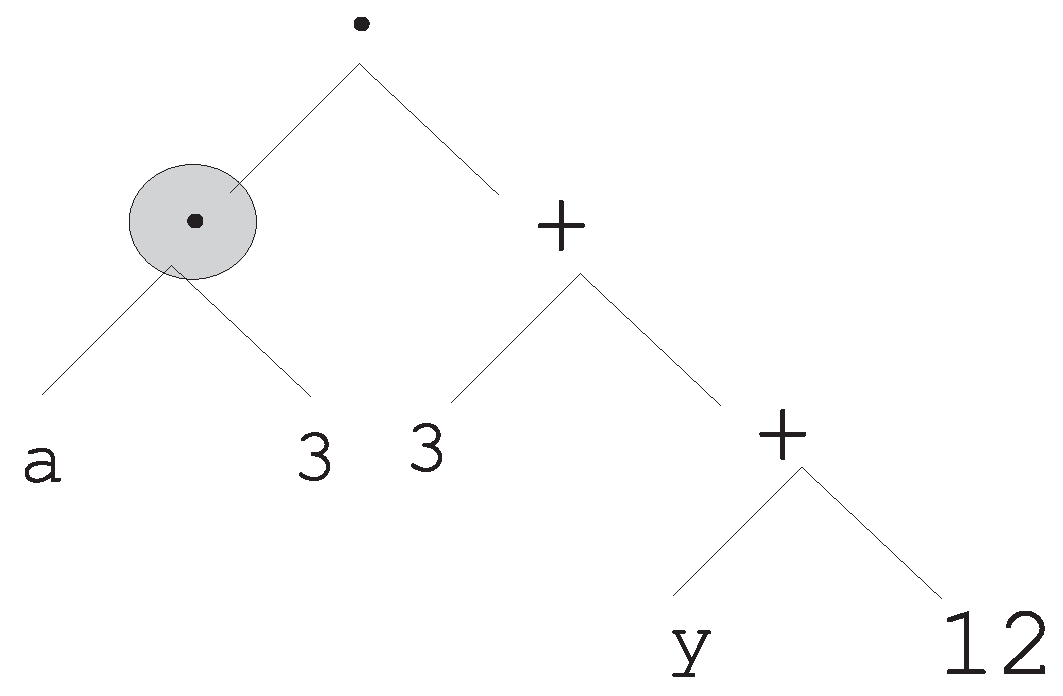
\includegraphics[width=\linewidth]{figs/gpparentbcrossover.eps}
			\end{columns}

			\begin{center}
				$\Downarrow$
			\end{center}

			\begin{columns}
 	   			\column{.5\textwidth}
					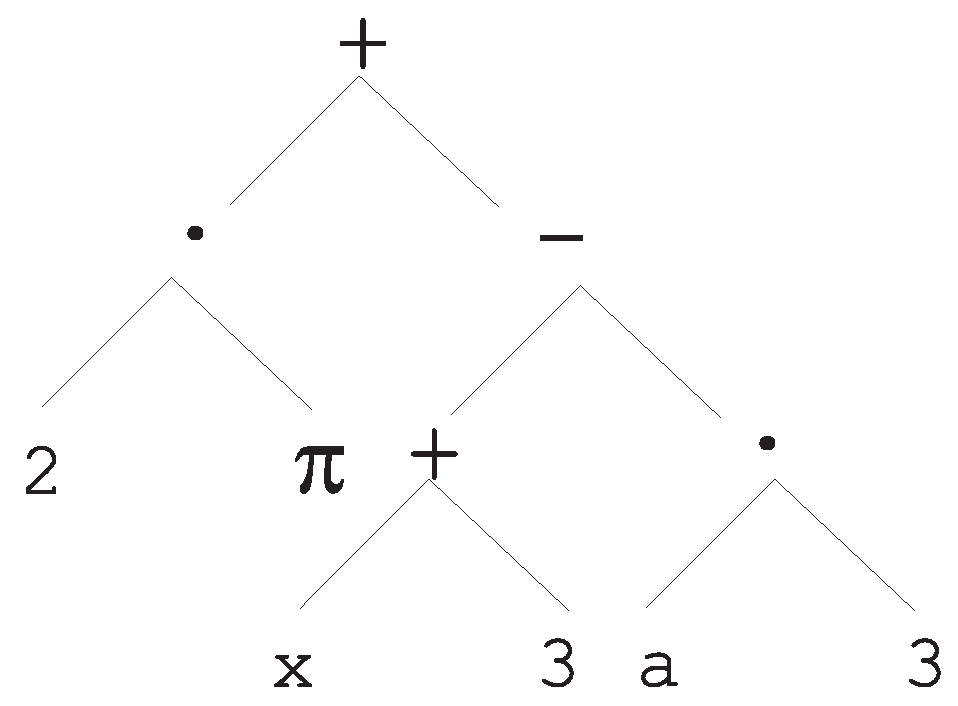
\includegraphics[width=\linewidth]{figs/gpchildacrossover.eps} 
 	   			\column{.02\textwidth}
					,
 	   			\column{.5\textwidth}
					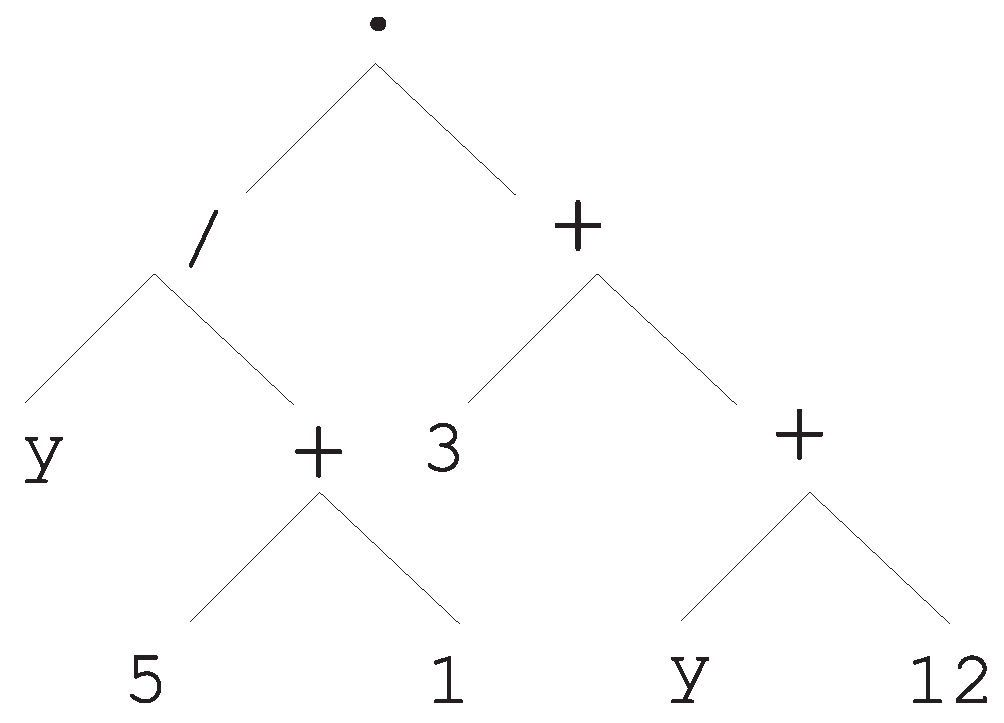
\includegraphics[width=\linewidth]{figs/gpchildbcrossover.eps}
			\end{columns}

	\end{columns}
\end{frame}

\begin{frame}{Genetic Programming}{Recombination (II)} 
	Alternative recombination operators
	\begin{itemize}
		\item Homologous crossover
		\item Uniform crossover
		\item Size-fair crossover
		\item Node replacement mutation (point mutation)
		\item Hoist mutation
		\item Shrink mutation
	\end{itemize}
\end{frame}

\subsection{Initialization}
\begin{frame}{Genetic Programming}{Initialization} 
	\vspace{-0.2cm}
    \begin{columns}
 	   \column{.70\textwidth}
		Three initialization methods
		\begin{itemize}
			\item \textbf{Full}. Introduces non-terminals nodes until max depth
			\item \textbf{Grow}. Introduces terminal or non-terminal with equal probability
			\item \textbf{Ramped half-n-half}. Applies full or grow with equal probability
		\end{itemize}

 	   \column{.30\textwidth}
		\begin{center}
			Full (D=2)\\
			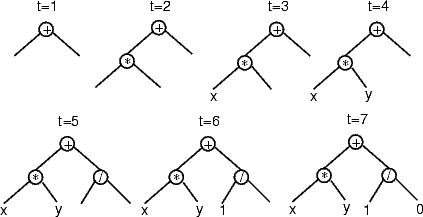
\includegraphics[width=\linewidth]{figs/full.jpg}\\
			\bigskip
			Grow (D=2)\\
			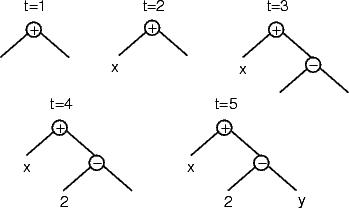
\includegraphics[width=\linewidth]{figs/grow.jpg}
		\end{center}
	\end{columns}
\end{frame}

\subsection{Bloat in Genetic Programming}
\begin{frame}{Genetic Programming}{Bloat in Genetic Programming} 
	\vspace{-0.5cm}
    \begin{columns}
 	   \column{.70\textwidth}
		\textbf{Code bloat}: Uncontrolled grow of tree sizes
		\begin{itemize}
			\item Intrinsic to variable-length representations
			\item Undesirable effects
			\item Perhaps, the worse problem in GP
		\end{itemize}

		Countermeasures
		\begin{itemize}
			\item Depth limitation in genetic operators
			\item Parsimony pressure
			\item Tree plunning
			\item Multiobjective techniques
		\end{itemize}

 	   \column{.30\textwidth}
		\begin{center}
			\includegraphics[width=\linewidth]{figs/depth-k2.eps}\\
			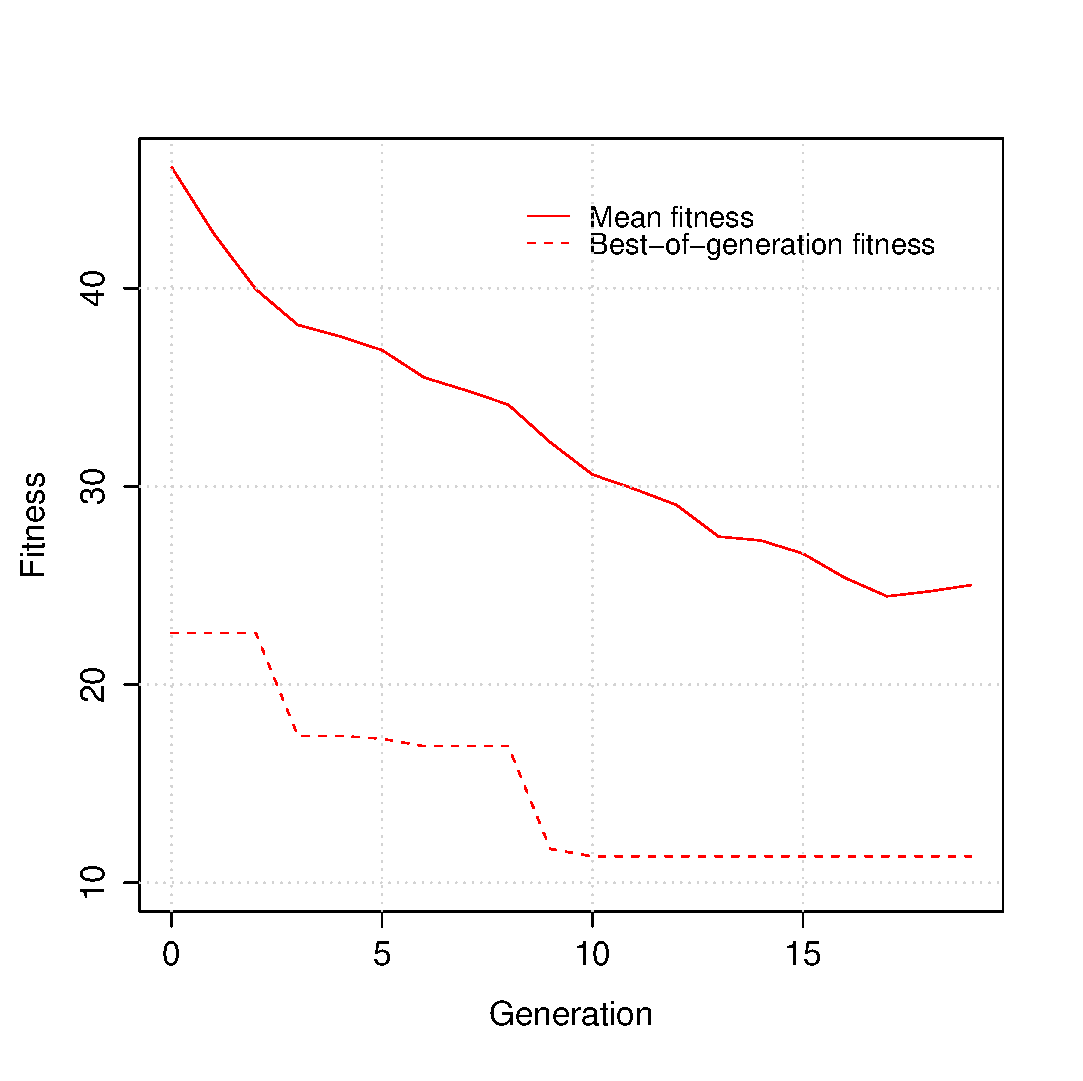
\includegraphics[width=\linewidth]{figs/fitness-k2.eps}
		\end{center}
	\end{columns}
\end{frame}

\begin{frame}[plain]{Genetic Programming}{Example of reporting} 
\scriptsize{
\begin{table}
	\centering
	\caption{Main parameters used to obtain the approximations for secrets $ID$ in the Genetic Tango attack against David-Prasad authentication protocol.  \label{tab:settings}}
	\begin{tabular}{clll} \hline 
	Parameter		& $ID$			\\ \hline
	Population		& 500			\\
	Generations		& 10			\\
	Terminal Set	& $A$, $B$, $D$, $E$, $F$, $P_{ID1}$, $P_{ID2}$	\\
	Function set	& And, or, xor	\\
	Fitness			& Hamming distance to secret\\
	Fitness tags	& 5				\\
	Fitness sessions& 100			\\
	Min. depth		& 1				\\
	Max. depth		& 3 			\\
	Selection		& Lexicographic tournament\\
	Tournament size	& 4				\\
	Crossover		& 0.9			\\
	Reproduction	& 0.1			\\
	Elitism size	& 1 			\\
	Terminals		& 0.1			\\
	Non terminals	& 0.9			\\
	Initialization  & Rampled H-H	\\
	\hline\end{tabular}
\end{table}
}
\end{frame}

\section{Evolution Strategies}
\subsection{Introduction}

\begin{frame}{Evolution Strategies}{Introduction (I)}
	Introduced by Rechenberg and Schwefel in the 60's
	\begin{itemize}
		\item Motivated by wing shape optimization
		\item Real-function optimization
	\end{itemize}
	ES properties
	\begin{itemize}
		\item Emphasis on mutation
		\item Mutation is gaussian noise
		\item Self-adaptation
	\end{itemize}
	\small{
	\begin{table}
	\centering
	\begin{tabular}{|c|l|} \hline 
	Representation		& Real-valued vectors	\\
	Recombination		& Discrete		\\
	Mutation			& Gaussian perturbation	\\
	Parent selection	& Uniform			\\
	Survivor selection 	& $(\mu,\lambda)$ or $(\mu+\lambda)$\\
	Speciality			& Self-adaptation\\
	\hline\end{tabular}
	\end{table}
	}
\end{frame}

\begin{frame}{Evolution Strategies}{Introduction (II)}
	Example of basic ES
	\begin{itemize}
		\item Representation: Vector of real values
		\item Recombination: Not used
		\item Mutation: Gaussian noise with \alert{step-size} $\sigma$
	\end{itemize}
	Adaptative $\sigma$ (\alert{1/5 rule})
	\begin{itemize}
		\item Theorerical foundations
		\item Based on the ratio of success mutations ($p_s$)
		\item After $k$ iterations a new $\sigma$ is computed
	\end{itemize}
	\begin{equation*}
 \sigma = 
   \begin{cases} 
      \sigma/c 		& \text{if } p_s > 1/5, \\
	  \sigma \cdot c & \text{if } p_s < 1/5, \\
	  \sigma		& \text{if } p_s = 1/5
	\end{cases}
	\end{equation*}
	where $0.817 \le c \le 1$ is a parameter
\end{frame}

\subsection{Representation}
\begin{frame}{Evolution Strategies}{Representation}
	Nowdays ES is usually self-adapted
	\begin{itemize}
		\item Step size ($\sigma$) is included in the genotype
		\item Evolution includes variables and parameters
	\end{itemize}
	One or more $\sigma$ values
	\begin{itemize}
		\item One  $\sigma$: $\big<\underbrace{x_1, x_2, ..., x_n}_{\bar{x}},\sigma\big>$
		\item Several: $\sigma : \big<\underbrace{x_1, x_2, ..., x_n}_{\bar{x}},
		\underbrace{\sigma_1, \sigma_2, ..., \sigma_{n_{\sigma}}}_{\bar{\sigma}}\big>$
	\end{itemize}
\end{frame}

\subsection{Mutation}
\begin{frame}{Evolution Strategies}{Mutation}
	%New values are computed as $x_i = x_i + N(0, \sigma)$
	%\begin{itemize}
%		\item $\sigma$ coevolves with the solutions
%	\end{itemize}
	Genetic operators to modify $\sigma$
	\begin{itemize}
		\item Mutation with one step size: 
		\begin{subequations}
		\begin{align*}
		x_i' = & x_i + N_i(0, \sigma')\\
		\sigma' = & \sigma \cdot e^{\cdot N(0, \tau)} \text{, } \tau \propto 1/\sqrt{n}
		\end{align*}
		\end{subequations}
		$\tau$ is analogous to learning rate in ANN
		\item Mutation with n step sizes:
		\begin{subequations}
		\begin{align*}
		x_i' = & x_i + N_i(0, \sigma_i)\\
		\sigma' = & \sigma \cdot e^{\cdot N(0, \tau')+N_i(0, \tau}
		\end{align*}
		\end{subequations}
		with $ \tau' \propto 1/\sqrt{2n}$  and $\tau \propto 1/\sqrt{2\sqrt{n}}$
	\end{itemize}
\end{frame}

\subsection{Recombination}
\begin{frame}{Evolution Strategies}{Recombination}
	Secondary operator in ES
	\begin{itemize}
		\item \textbf{Discrete recombination}. Like uniform crossover in GA
		\item \textbf{Intermediate recombination}. Like arithmetic crossover in GA
	\end{itemize}
	ES tends to use \textbf{global recombination}
	\begin{itemize}
		\item More than two parents
	\end{itemize}
\end{frame}

\subsection{Parent and survivor selection}
\begin{frame}{Evolution Strategies}{Parent and survivor selection}
	The whole population is seen as parent
	\begin{itemize}
		\item Select individual with uniform probability
		\item No selective pressure in parent selection
	\end{itemize}
	After creating the offspring, the $\lambda$ fittests individuals are selected
	\begin{itemize}
		\item Deterministic procedure
	\end{itemize}
	Two selection mechamisms depending on who can be selected
	\begin{itemize}
		\item \textbf{$(\mu, \lambda)$ selection}. Only the offpring.  
		\item \textbf{$(\mu + \lambda)$ selection}. Parents and offpring
	\end{itemize}
	$(\mu, \lambda)$ selection is more popular
\end{frame}


\end{document}
